\let\negmedspace\undefined
\let\negthickspace\undefined
\documentclass[journal]{IEEEtran}
\usepackage[a5paper, margin=10mm, onecolumn]{geometry}
%\usepackage{lmodern} % Ensure lmodern is loaded for pdflatex
\usepackage{tfrupee} % Include tfrupee package

\setlength{\headheight}{1cm} % Set the height of the header box
\setlength{\headsep}{0mm}     % Set the distance between the header box and the top of the text

\usepackage{gvv-book}
\usepackage{gvv}
\usepackage{cite}
\usepackage{amsmath,amssymb,amsfonts,amsthm}
\usepackage{algorithmic}
\usepackage{graphicx}
\usepackage{textcomp}
\usepackage{xcolor}
\usepackage{txfonts}
\usepackage{listings}
\usepackage{enumitem}
\usepackage{mathtools}
\usepackage{gensymb}
\usepackage{comment}
\usepackage[breaklinks=true]{hyperref}
\usepackage{tkz-euclide} 
\usepackage{listings}
% \usepackage{gvv}                                        
\def\inputGnumericTable{}                                 
\usepackage[latin1]{inputenc}                                
\usepackage{color}                                            
\usepackage{array}                                            
\usepackage{longtable}                                       
\usepackage{calc}                                             
\usepackage{multirow}                                         
\usepackage{hhline}                                           
\usepackage{ifthen}                                           
\usepackage{lscape}
\begin{document}

\bibliographystyle{IEEEtran}
\vspace{3cm}

\title{1/1.5/36}
\author{EE24BTECH11040 - Mandara Hosur}
% \maketitle
% \newpage
% \bigskip
{\let\newpage\relax\maketitle}

\renewcommand{\thefigure}{\theenumi}
\renewcommand{\thetable}{\theenumi}
\setlength{\intextsep}{10pt} % Space between text and floats


\numberwithin{equation}{enumi}
\numberwithin{figure}{enumi}
\renewcommand{\thetable}{\theenumi}


\textbf{Question:}\\
Point $\vec{P}(x,4)$ lies on the line segment joining the points $\vec{A}(-5,8)$ and $\vec{B}(4,-10)$. Find the ratio in which point $\vec{P}$ divides the line segment $AB$. Also, find the value of $x$.
\\
\textbf{Solution:}
\begin{table}[h!]    
  \centering
  \begin{tabular}[12pt]{ |c| c|}
    \hline
    \textbf{Given Points} & \textbf{Description} \\ 
    \hline
    $\brak{-2,3,5}$ & Point $\vec{A}$ \\
    \hline 
    $\brak{1,2,3}$ & Point $\vec{B}$\\
    \hline
    $\brak{7,0,-1}$ & Point $\vec{C}$\\
    \hline 
    \end{tabular}

  \caption{Given Information}
  \label{Table 1}
\end{table} \\
To find $x$: $$\vec{A}-\vec{B}=r\brak{\vec{A}-\vec{P}}$$ \\
$$\implies \myvec{-5\\8} - \myvec{4\\-10} = r\brak{\myvec{-5\\8} - \myvec{x\\4}}$$\\
$$\implies \myvec{-9\\18} = r\myvec{-5-x\\4}$$
$$\implies 18=4r$$
$$\implies r=\frac{18}{4}=\frac{9}{2}$$
Also, $$9=r\brak{5+x}$$
$$\implies 9=\frac{9}{2}\brak{5+x}$$
$$\text{or, }x=-3$$
To find k: $$\vec{P}=\frac{1}{1+k}\brak{\vec{A}+k\vec{B}}$$
$$\myvec{-3\\4}=\frac{1}{1+k}\brak{\myvec{-5\\8}+k\myvec{4\\-10}}$$
$$\implies \myvec{-3\\4}=\frac{1}{1+k}\myvec{4k-5\\8-10k}$$
$$\text{or, }k=\frac{2}{7}$$

\begin{figure}[h]
    \centering
    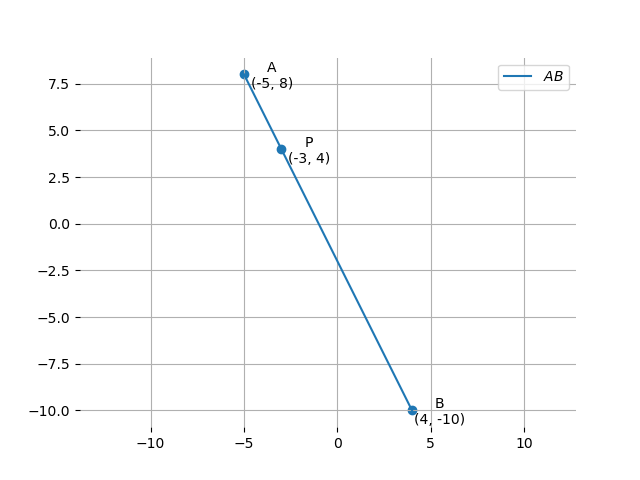
\includegraphics[width=\columnwidth]{figs/fig.png}
    \caption{Plot of line segment $AB$ along with point $\vec{P}$}
 \end{figure}

\end{document}
